
%Batteries are important

%Use EM to analyze them

%In particular EELS is good

%Want simulations, use DFT
 
%Want better simulations improve core hole method
\setcitestyle{numbers,open={[},close={]}}

The study of lithium materials has become increasingly relevant over the years.  In particular, the field has been driven by the need to develop improved battery materials.  This drive has come from an array of fields, amongst others, electric vehicles and portable electronics desiring longer lifetimes and faster charging.  All aspects of batteries are currently being improved including capacity, charge density, and charge/discharge rates.  As well as performance, other features such as safety and the ability to reuse or recycle battery materials are also growing fields.  \\
In the realm of performance, lithium ion batteries offer a wide range of advantages.  Lithium is the third element on the periodic table and consequently offers very high charge densities.  This allows for batteries to become smaller and lighter without sacrificing lifetime.  Additionally, lithium's lightweight nature make it highly mobile which is an attractive feature for increasing maximal discharge rate.  Finally, as an alkali earth metal with a single weakly bound valence electron, lithium is highly electropositive  which allows lithium ion batteries to achieve higher operating voltages than alternatives such as nickle-cadmium or lead-acid batteries.  These potential performance advantages are illustrated in Fig \ref{ragone}.
\\

\begin{figure}
	\centering
	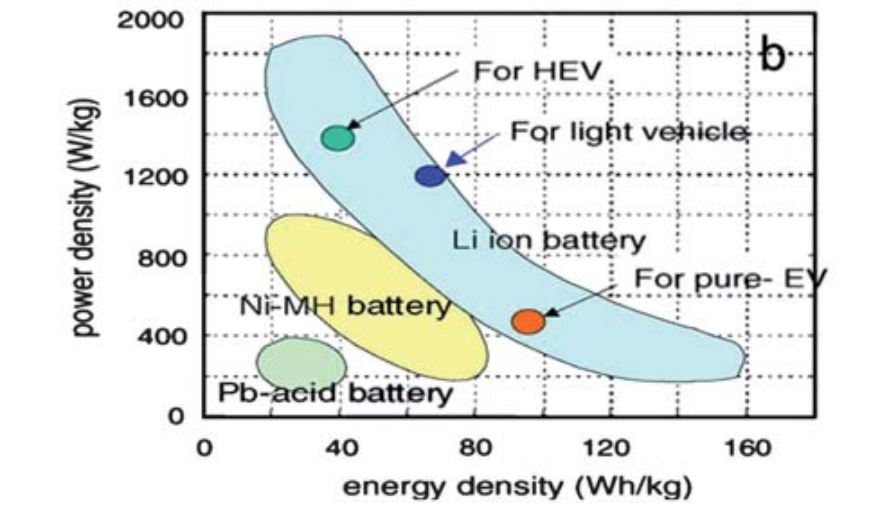
\includegraphics[scale=0.3]{ragone_plot}
	\caption{Plot illustrating the the power and energy densities achievable by three types of battery, as well as the minimum requirements for various types of electric vehicle, including hybrid electric vehicles (HEV), plug in hybrids (light vehicle). From \cite{etacheri_challenges_2011} }
	\label{ragone}
	
\end{figure}
The pursuit of developing new and improved battery materials has shifted the focus of analysis towards studying the microstructure of materials. The ability to identify crystal structure and composition has become an essential element to understanding and tailoring material properties.  On this front, electron microscopy has become a central technique to this effort  \cite{inkson_2_2016}.  Rapidly improving technology, the possibility of atomic level resolution, coupled with the increasing accessibility have made electron microscopy one of the most prevalent techniques for studying nanoscale features in materials.  Here, however lithium is at odds with the method.  Novel battery materials are increasingly intricate and lithium's lightness and easy to ionize nature make it particularly sensitive to electron beams, complicating analysis.  Additionally, as the third element, it lies outside the ranges of many conventional theories.  These properties make electron energy loss spectroscopy (EELS), a low dosage technique that is well suited for light elements such as lithium, attractive for battery material analysis   \cite{Egerton}.  However, EELS results have been historically qualitative and require strong theoretical support to be analyzed.  The theoretical support is all the more essential in dealing with novel lithium materials that have limited sample life.   
\\
The theoretical support for EELS can come from a number of methods, however, the most prevalent of these are based in density functional theory (DFT), a first principles approach that requires only the locations of atoms in a crystal to determine material properties \cite{ks_1965}.  Here too, results have been limited to qualitative findings, further complicated by lithium's lightweight nature which also poses challenges to theoretical approaches.  The work performed in this thesis was to address some of the issues facing DFT methods concerning EELS of lithium.  In particular, an improved method of calculating electron screening was implemented to improve the core hole approximation used to handle excitonic effects.  
\\

The outline of this thesis is as follows: in Chapter 2 we will begin with an overview of EELS, DFT and theoretical EELS calculations.  Chapter 3 will describe the improved method developed in this work, and Chapter 4 will apply the method to a number of lithium materials.  Chapter 5 will conclude the results and address future work.


